\documentclass[]{article}
\usepackage[utf8]{inputenc}
\usepackage{url}
\usepackage{geometry}
\usepackage{floatflt} 
\usepackage{float} 
\usepackage{wrapfig}
\usepackage{graphicx}
\geometry{verbose,a4paper,tmargin=15mm,bmargin=15mm,lmargin=15mm,rmargin=15mm}
%opening
\date{Mi, 04.06.2014}
\title{Web Programming Weeks SS14 \\Projektwoche}
\author{Handout für}

\begin{document}

\maketitle

\section{Entwicklungs-Infrastruktur}
\subsection{Einrichten der Entwicklungsumgebung}
Folgen Sie den Anweisungen des \textit{Working-Sheets} (\url{http://bit.ly/1rGoZsy}) der iCampus-Gruppe zum Einrichten Ihrer Entwicklungsumgebung.
\subsection{Lokale PHP-Umgebung einrichten}
Für Ihre lokale PHP-Umgebung laden Sie sich XAMPP unter \url{https://www.apachefriends.org/de/index.html} herunter und installieren es auf Ihrem Rechner. XAMPP beinhaltet neben dem Apache Server zur lokalen Übersetzung von PHP-Skripten einen MySQL-Server, welcher für die Verwendung von Joomla benötigt wird.\\
\\
Um PHP-Dateien zu übersetzen müssen Sie den Apache-Server über das Control-Panel starten. Achten Sie hierbei darauf, dass die Ports 80 und 443 nicht von einer anderen Anwendung (z.B. Skype) blockiert sind.\\
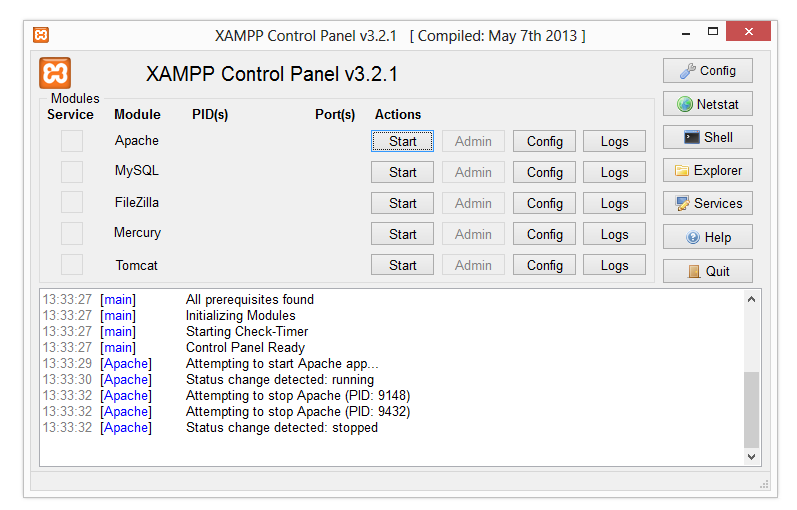
\includegraphics[width=0.8\textwidth]{XAMPP_controlpanel}\\
Um PHP-Skripte auszuführen müssen sich diese innerhalb des Ordners \textit{$<$Pfad zu XAMPP-Ordner $>$}\textbackslash{}htdocs\textbackslash{} befinden. Zur Ausführung muss das jeweilige Skript nur im Browser aufgerufen werden (\textbf{\textit{localhost}} nicht vergessen):\\
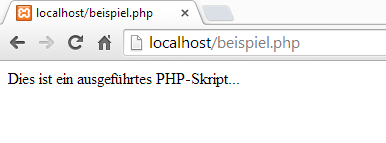
\includegraphics{php_Script}
\subsection{Versionsverwaltung mit Gitorious}
\begin{wrapfigure}{r}{40mm}
  \vspace{-80pt}
  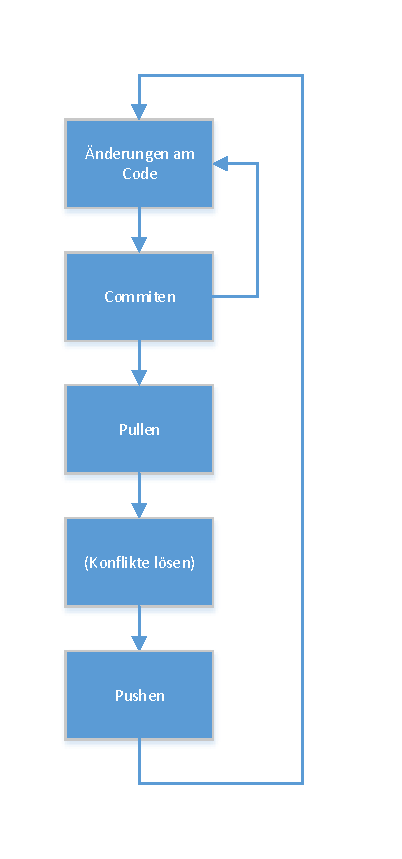
\includegraphics[width=0.33\textwidth]{GitCycle}
  \label{fig:GitCycle}
  \vspace{-120pt}
\end{wrapfigure}

Gitorious bietet eine Open-Source-Infrastruktur zur  Versionsverwaltung von Dateien eines Projekts. Basierend auf Git kann dadurch kollaborativ an einem Projekt gearbeitet werden. Folgende Features können genutzt werden:
\begin{itemize}
\item Veröffentlichen von Projekten mit Wiki
\item Verwaltung von Repositories innerhalb von Projekten
\item Übersicht über Aktivitäten in Projekten und von Entwicklern
\item Teambildung und Entwicklerprofile
\end{itemize}
Das klonen eines Repositories bewirkt das man eine exakte lokale Kopie auf seinem Rechner hat. Wenn Änderungen an den Datei gemacht wurden werden diese committed. Damit sind die Änderungen erstmal im lokalen Repository festgehalten. Damit andere die Änderungen sehen können muss man seine Commits in das zentrale Repository pushen. Wenn man Änderungen von anderen haben möchte pullt man diese und hat diese dann auch lokal. Dabei können so genannte Merge-Konflikte auftreten. Bei der Lösung des Konflikts hilft einem die IDE. Der normale Ablauf sieht wie in der Abbildung aus.\\

\subsection{Projektmanagement mit Redmine}
\begin{itemize}
\item \url{https://scm.thm.de/redmine}
\item Menüpunkt \textit{Backlogs} innerhalb eines Projektes öffnet Scrum-Ansicht (Product und Sprint Backlogs)
\item Innerhalb der Backlog-Ansicht können nun für jeden Sprint das Taskboard (Aufgabenliste), sowie der Burndown-Chart geöffnet werden.\\
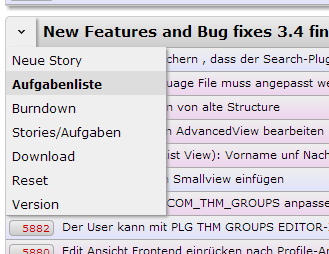
\includegraphics[width=0.33\textwidth]{Backlogs.png}
\item Tasks können in der Backlog-Ansicht einfach per Drag \& Drop zwischen Product und Sprint Backlogs verschoben werden
\end{itemize}
\section{Joomla}
Die Aufgabenstellungen in diesem Kapitel sollen als Einarbeitung in Joomla (2.5 \& 3.2) dienen. Als Hilfsmittel kann das iCampus Working Sheet genutzt werden (\url{http://bit.ly/1rGoZsy}) genutzt werden. 
\subsection{Joomla 2.5}
\begin{enumerate}
\item \textbf{Joomla 2.5 herunterladen \& installieren} \newline Hinweis: Nutzen Sie dazu die Anleitung im WPW Skript (2.4 Joomla! Installation)
\item \textbf{Legen Sie sich selbst als neuen Benutzer an und weisen Sie diesem der Gruppe "Registered" zu} \newline
Hinweis: Backend-URL: localhost/$ < $Joomla-Verzeichnisname-im-htdocs-Ordner$ > $/administrator. \\
Die Zuweisung zu einer Gruppe kann direkt beim Erstellen des Benutzer durchgeführt werden.
\item \textbf{Notieren Sie sich den Namen des Templates welches im Frontend benutzt wird} \newline
Hinweis: Erweiterungen-$ > $Templates
\item \textbf{Erstellen Sie ein neues Menü und weisen Sie diesem einem Menü-Modul hinzu} \newline
Hinweis: Menüs-$ > $Neues Menü. Schauen Sie sich die Modulinstanz mit dem Namen "Main Menü" an (Erweiterungen-$>$Module). Die Position des Moduls bestimmt an welcher Stelle das Menü auf der Seite angezeigt wird (Rechts oben können die Positionen nach Template gefiltert werden!).
\item \textbf{Erstellen Sie einen Menüpunkt (Menütyp: Benutzerprofil bearbeiten) im neuen Menü, den nur Benutzer in der Gruppe "Special" sehen können!} \newline
Hinweis: Menüs-$ > $Neues Menü. Im neuen Menü "Neuen Menüeintrag" erstellen.
\item \textbf{Schauen Sie sich den neuen Menüpunkt im Frontend an. Können Sie das Menü sehen, wenn sie: nicht eingeloggt sind/mit ihrem eigenen Account eingeloggt sind/als Administrator eingeloggt sind?} \newline
Hinweis: Frontend-URL: localhost/$ < $Joomla-Verzeichnisname-im-htdocs-Ordner$ > $ 
\item \textbf{Ändern Sie den Menüpunkt so ab dass auch Benutzer in der Gruppe "Registered" den Eintrag sehen können.}
\item \textbf{Erstellen Sie einen neuen Menüpunkt (Menütyp: Kategorieblog) welcher die Beiträge einer Kategorie darstellt und für jeden sichtbar ist. (Schauen Sie sich das Ergebnis im Frontend an.)} \newline
Hinweis: Beachten Sie die erforderlichen Einstellungen dieser View. Weitere Kategorien können unter Inhalt-$>$Kategorien hinzugefügt werden.
\item \textbf{Erstellen Sie zwei neuen Beiträge für die Kategorie welche Sie in der vorherigen Aufgabe bei "Erforderlichen Einstellungen" angegeben haben. (Schauen Sie sich das Ergebnis im Frontend an.)} \newline
Hinweis: Inhalt-$>$Beiträge. 
\item \textbf{Editieren Sie den ersten Beitrag so dass Benutzer in der Gruppe "Registered", den Beitrag editieren können.} \newline
Hinweis: Im Beitrag die Beitragsberechtigungen müssen geändert werden. Berechtigungen können an vielen verschiedenen Stellen in Joomla gesetzt werden, zum Beispiel auch für Kategorien.
\item \textbf{Erstellen Sie eine neue Instanz des Suchmoduls (Modultyp: Suchen)} \newline
Hinweis: Erweiterungen-$>$Module->Neu. Position nicht vergessen!
\item \textbf{Suchen Sie im Frontend nach ihrem Beitrag} \newline
\end{enumerate}
\subsection{Joomla 3.2}
\begin{enumerate}
\item \textbf{Führen Sie die vorigen Schritte (Joomla 2.5) in Joomla 3.2 durch (läuft ähnlich wie in Joomla 2.5 ab, sieht nur ein wenig anders aus)}
Hinweis: Tutoren fragen, falls es Probleme gibt.
\end{enumerate}
\section{PHP}
\subsection{PHP - Onlinekurs}
Zur Einarbeitung in die Programmiersprache PHP, folgen Sie dem beigefügten Link um einen Onlinekurs der \textbf{\textit{codecademy}} zu absolvieren:
\begin{list}{}{}
\item \url{http://www.codecademy.com/de/tracks/php}
\end{list}
Tipp: Um ihren Fortschritt zu speichern, sollten Sie sich einen Account anlegen.
\subsection{Lokale Ausführung von PHP-Skripten}
\begin{enumerate}
\item Starten Sie Ihren lokalen Apache Server (XAMPP).
\item Erstellen Sie nun lokal eine PHP-Datei \textit{register.php}, welche beim Aufruf im Browser ein Registrierungs-Formular mit Absenden-Button darstellt. 
\item Rufen Sie die Datei in Ihrem Browser auf.
\item Nach der Eingabe der Daten soll der Benutzer auf den Absenden-Button klicken, woraufhin eine weitere Datei aufgerufen werden soll, welche wiederum die eingegebenen Daten im Browser formatiert darstellen soll. Erstellen Sie dafür eine Datei \textit{show\_register\_data.php} und passen Sie Datei Register entsprechend an.
\item Rufen Sie nun erneut die Datei register.php in Ihrem Browser auf um den Registrierungsvorgang mit beiden Skripten zu testen.
\end{enumerate}
\end{document}
